\chapter{REST - Representational State Transfer}
\section{Definizione}
REST è uno \textbf{stile architettonico} per i sistemi distribuiti.

\begin{itemize}
    \item \uline{Le risorse} so \textbf{identificate da URI}.
    \item \uline{Le risorse} vengono manipolate attraverso le loro \textbf{rappresentazioni} (possono esistere più rappresentazioni di una risorsa).
    \item \uline{Comunicazione tramite messaggi} che sono \textbf{autodescrittivi e senza stato}.
    \item \uline{Lo stato dell'applicazione} evolve per mezzo della \textbf{manipolazione} delle risorse da parte dei client.
    \item \uline{Hypermedia} è il modo che il server ha per \textbf{guidare il comportamente del client}.
\end{itemize}

\section{Risorse e Interfaccia unifome}
\subsection{Risorse}
Una risorsa è una qualsiasi informazione che può essere nominata.
\begin{itemize}
    \item Le risorse di solito cambiano con l'interazione con il client.
    \item Le risorse hanno \textbf{identificatori}
    
    es:\texttt{unimib.it/\{matricola\}/pianoStudio}, \{matricola\} è chiamato \uline{path parameter}.
\end{itemize}

\subsection{Interfaccia uniforme}
\texttt{RESTful} prevede quattro operazioni \texttt{HTTP}
\begin{table}[h]
    \centering
    \begin{tabularx}{\textwidth}{|l|X|}
    \hline
    \textbf{Operazione} & \textbf{Descrizione} \\ \hline
    PUT & Modifica una risorsa / Nuovo stato \\ \hline
    POST & Crea una nuova risorsa \\ \hline
    GET & Recupera lo stato di una risorsa \\ \hline
    DELETE & Elimina una risorsa \\ \hline
    \end{tabularx}
\end{table}

\textbf{\uline{I messaggi \texttt{REST} sono completamente auto-descrittivi}}, contengono tutti i metadati necessari per la loro interpretazione, senza fare affidamento su contensto di sessione esterno.

\textbf{\uline{L'esecuzione è stateless}}, dopo ogni operazione il componente dimentica tutto del chiamante, rendendo le operazioni idempotenti e semplificando la scalabilità del sistema.

\section{Statelessness}
\begin{itemize}
    \item Ogni richiesta del client al server deve contenere tutte le informazioni necessarie a comprendere la richiesta e \textbf{\uline{non può sfruttare alcun contesto memorizzato sul server}}.
    \item La mancanza di stato richiede \textbf{messaggi autodescrittivi}.
\end{itemize}

\section{Cacheability}
La Cacheability è una proprietà fondamentale delle architettura \texttt{REST} e indica la \textbf{capacit delle risposte \texttt{HTTP} di essere memorizzate in cache} da client, proxy, gateway o CDN, al fine di migliorare l'efficienza, ridurre il carico sui server e diminuri la latenza percepita.

\vspace{\baselineskip}

La cacheability richiede un sistema a livelli:
\begin{itemize}
    \item Almeno un livello di cache.
    \item Nella cache è memorizzata l'ultima rappresentazione di una risorsa.
    \item Una cache viene invalidata quando viene modificato lo stato della risorsa (\texttt{PUT, DELETE}).
    \item \uline{\textbf{Vengono memorizzati nella cache solo le risposte ai \texttt{GET}}}.
\end{itemize}

\begin{figure}[H]
    \centering
    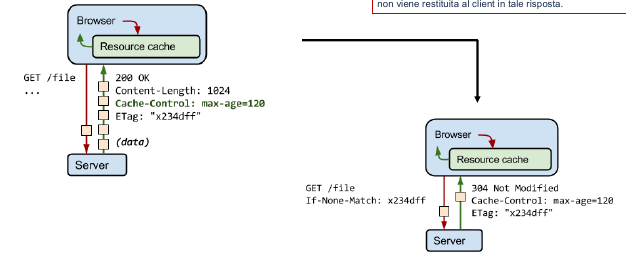
\includegraphics{figures/Schermata_20260514_104115.png}
\end{figure}

\subsection{Header utilizzati per il cache-controll}
\begin{table}[H]
\centering
\begin{tabularx}{\textwidth}{|l|X|}
\hline
\textbf{Intestazione} & \textbf{Proprietà} \\ \hline
Expires & Data HTTP. Mantenere in cache fino alla scadenza \\ \hline
Cache-Control: max-age & Un secondi. Mantenere in cache per il tempo indicato \\ \hline
Cache-Control: s-maxage & Secondi. Come sopra, ma solo per i proxy \\ \hline
Cache-Control: public & La risorsa può essere salvata in una cache condivisa \\ \hline
Cache-Control: no-cache & La risorsa può essere memorizzata nella cache, ma deve essere convalidata dal server di origine prima di ogni riutilizzo \\ \hline
Cache-Control: no-store & Non memorizzare nella cache \\ \hline
Cache-Control: must-revalidate & La risorsa può essere memorizzata in cache e riutilizzata quando è "fresca". Se diventa stantia (stale), deve essere convalidata con il server di origine prima di essere riutilizzata. \\ \hline
Cache-Control: proxy-revalidate & Come sopra, ma solo per i proxy \\ \hline
\end{tabularx}
\end{table}

\section{Stato dell'applicazone}
Nel contesto \texttt{REST}, lo \textbf{stato dell'applicazione} rappresenza \uline{il "percorso" del client nel sistema}: la sequenza di risorsa e interazioni attraversate durante l'uso dell'applicazione.

\begin{itemize}
    \item È \textbf{gestito dal client}.
    \item Include le risorse richieste, link seguiti, dati ricevuti e modificati.
    \item Si evolve \uline{man mano che il client invia richieste} e riceve risposte che includono link e altre risorse.
\end{itemize}

\begin{figure}[H]
    \centering
    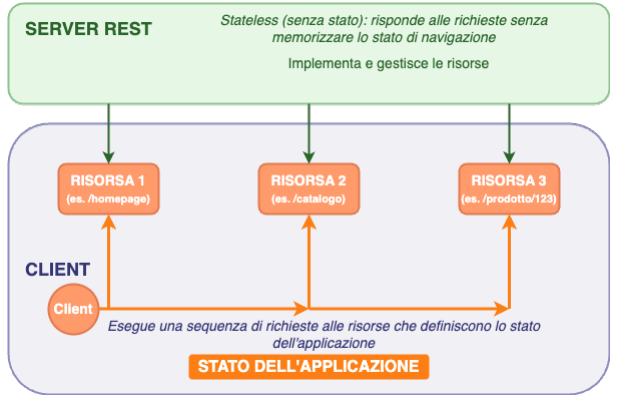
\includegraphics[scale=0.8]{figures/Schermata_20260514_105231.png}
\end{figure}

\subsection{Hypermedia control}
I client devono seguirie i link forniti dal server, i link devono essere "classificati" con un significato semantico in modo che un client inteliggete sappia a cosa punta un il link.

\subsection{Esempio : Gestione del curriculm universitario}
\begin{itemize}
    \item\textbf{\texttt{GET unimib.it/\{matricola\}}} : restituisce informazioni sullo studente e l'elenco di altre risorse collegate:
    \begin{itemize}
        \item \texttt{nome, cognome, data-di-nascita, etc.}
        \item \texttt{unimib.it/\{matricola\}/badges}
        \item \texttt{unimib.it/\{matricola\}/pianostudio}
        \item \texttt{unimib.it/\{matricola\}/storicorate}
    \end{itemize}
    
    \item \textbf{\texttt{GET unimib.it/\{matricola\}/pianostudio}} :
    \begin{itemize}
        \item \textbf{GET} per ottenere l'elenco degli esami a cui lo studente è iscritto,
        \item \textbf{POST} per iscriversi a un esame,
    \end{itemize}
    
    \item \textbf{\texttt{GET unimib.it/\{matricola\}/pianostudio/\{codice\}}} :
    \begin{itemize}
        \item \textbf{GET} per ottenere informazioni sull'esame a cui lo studente è iscritto
        \item \textbf{PUT} per modificare la registrazione dell'esame,
        \item \textbf{DELETE} per eliminare la registrazione dell'esame
    \end{itemize}
\end{itemize}

\begin{lstlisting}
HTTP/1.1 200 OK
Content-Type: application/vnd.unimib.student+json
Content-Length: ...

{
  "studente": {
    "matricola": "123456",
    "nome": "Mario",
    "cognome": "Rossi",
    "data_di_nascita": "2000-04-15",
    "email": "mario.rossi@unimib.it",
    "_links": {
      "self": {
        "href": "unimib.it/123456"
      },
      "badges": {
        "href": "unimib.it/123456/badges"
      },
      "piano_studio": {
        "href": "unimib.it/123456/pianostudio"
      },
      "storico_rate": {
        "href": "unimib.it/123456/storicorate"
      }
    }
  }
}
\end{lstlisting}